
\chapter{何西阿書}

\section{先知的婚姻和子女的预表 1-3}

\subsection{先知服事的时期 1:1}
當烏西雅、約坦、亞哈斯、希西家做\underline{猶大王}，約阿施的兒子耶羅波安做\underline{以色列王}的時候，耶和華的話臨到備利的兒子\underline{何西阿}。

 
\subsection{先知儿女名字的启示 1:2-2:23}
\subsubsection{主命先知娶淫妇为妻 1:2-3}
耶和華初次與何西阿說話，對他說：「你去娶淫婦為妻，也收那從淫亂所生的兒女，因為這地大行淫亂，離棄耶和華。」 3 於是，何西阿去娶了滴拉音的女兒歌篾。

\subsubsection{歌篾生兒子耶斯列 1:3-5}
這婦人懷孕，給他生了一個兒子。 4 耶和華對何西阿說：「給他起名叫\underline{耶斯列(神栽種)}，因為再過片時，我必討耶戶家在耶斯列殺人流血的罪，也必使以色列家的國滅絕。 5 到那日，我必在耶斯列平原折斷以色列的弓。」


\subsubsection{歌篾生女兒羅路哈瑪 1:6-7}
\begin{itemize}
\itemsep-.45em  
\item 歌篾又懷孕，生了一個女兒。
\item 耶和華對何西阿說：給她起名叫\underline{羅路哈瑪（不蒙憐憫）}
\begin{itemize}
\itemsep-.45em  
\item 因為我必不再憐憫以色列家，決不赦免他們
\item 我卻要憐憫猶大家，使他們靠耶和華他們的神得救，不靠弓、刀、爭戰、馬匹與馬兵得救
\end{itemize}
\end{itemize}

\subsubsection{歌篾復生兒子羅阿米 1:8-9}
\begin{itemize}
\itemsep-.45em  
\item 歌篾給羅路哈瑪斷奶以後，又懷孕，生了一個兒子
\item 耶和華說：給他起名叫\underline{羅阿米（非我民）}
\begin{itemize}
\itemsep-.45em  
\item 因為你們不做我的子民
\item 我也不做你們的神。 
\end{itemize}
\end{itemize}

\subsubsection{对以色列民的预言 1:10-2:23}
%\subsubsubsection{預言耶斯列的日子猶大與以色列復興 1:10-2:1}
%然而，以色列的人數必如海沙，不可量，不可數。從前在什麼地方對他們說『你們不是我的子民』，將來在那裡必對他們說『你們是永生神的兒子』。 11 猶大人和以色列人必一同聚集，為自己立一個首領，從這地上去(從被擄之地上來)，因為耶斯列的日子必為大日。你們要稱你們的弟兄為阿米（我民），稱你們的姐妹為路哈瑪（蒙憐憫）。

\begin{itemize}
\itemsep-.45em  
\item 預言耶斯列的日子猶大與以色列復興 1:10-2:1
\begin{itemize}
\itemsep-.45em  
\item 然而，以色列的人數必如海沙，不可量，不可數。
\item 從前在什麼地方對他們說『你們不是我的子民』，將來在那裡必對他們說『你們是永生神的兒子』。 
\item 猶大人和以色列人必一同聚集，為自己立一個首領，從這地上去（從被擄之地上來），因為耶斯列的日子必為大日
\item 「你們要稱你們的弟兄為阿米（我民），稱你們的姐妹為路哈瑪（蒙憐憫）。
\end{itemize}
\item 以色列的罪 2:2-2:13
\begin{itemize}
\itemsep-.45em  
\item 「你們要與你們的母親大大爭辯，因為她不是我的妻子，我也不是她的丈夫。叫她除掉臉上的淫像和胸間的淫態， 3 免得我剝她的衣服，使她赤體，與才生的時候一樣，使她如曠野，如乾旱之地，因渴而死。 4 我必不憐憫她的兒女，因為他們是從淫亂而生的。 
\item 5 他們的母親行了淫亂，懷他們的母做了可羞恥的事，因為她說：『我要隨從所愛的，我的餅、水、羊毛、麻、油、酒都是他們給的。』 6 因此，我必用荊棘堵塞她的道，築牆擋住她，使她找不著路。 7 她必追隨所愛的卻追不上，她必尋找他們卻尋不見，便說：『我要歸回前夫，因我那時的光景比如今還好。』
\item 8 「她不知道是我給她五穀、新酒和油，又加增她的金銀，她卻以此供奉（製造）巴力。 9 因此，到了收割的日子，出酒的時候，我必將我的五穀、新酒收回，也必將她應當遮體的羊毛和麻奪回來。 10 如今我必在她所愛的眼前顯露她的醜態，必無人能救她脫離我的手。 11 我也必使她的宴樂、節期、月朔、安息日，並她的一切大會，都止息了。 12 我也必毀壞她的葡萄樹和無花果樹，就是她說『這是我所愛的給我為賞賜』的。我必使這些樹變為荒林，為田野的走獸所吃。 13 我必追討她素日給諸巴力燒香的罪，那時她佩戴耳環和別樣裝飾，隨從她所愛的，卻忘記我。這是耶和華說的。
\end{itemize}
\item 神勸導以色列悔改,受罰之後復蒙眷愛 2:14-2:23
\begin{itemize}
\itemsep-.45em  
\item 「後來我必勸導她，領她到曠野，對她說安慰的話。 15 她從那裡出來，我必賜她葡萄園，又賜她亞割谷作為指望的門。她必在那裡應聲（歌唱），與幼年的日子一樣，與從埃及地上來的時候相同。 16 耶和華說：那日你必稱呼我伊施（我夫），不再稱呼我巴力（我主）。 17 因為我必從我民的口中除掉諸巴力的名號，這名號不再提起。 18 當那日，我必為我的民，與田野的走獸和空中的飛鳥並地上的昆蟲立約。又必在國中折斷弓刀，止息爭戰，使他們安然躺臥。 19 我必聘你永遠歸我為妻，以仁義、公平、慈愛、憐憫聘你歸我， 20 也以誠實聘你歸我，你就必認識我耶和華。

\item 21 「耶和華說：那日我必應允，我必應允天，天必應允地， 22 地必應允五穀、新酒和油，這些必應允耶斯列（神栽種）民。 23 我必將她種在這地，素不蒙憐憫的，我必憐憫，本非我民的，我必對他說『你是我的民』，他必說『你是我的神』。」
\end{itemize}
\end{itemize}

\subsection{先知淫妻的启示——丈夫之愛 3:1-5}
耶和華對我說：「你再去愛一個淫婦，就是她情人所愛的；好像以色列人，雖然偏向別神，喜愛葡萄餅，耶和華還是愛他們。」 2 我便用銀子十五舍客勒，大麥一賀梅珥半，買她歸我。 3 我對她說：「你當多日為我獨居，不可行淫，不可歸別人為妻，我向你也必這樣。」 4 以色列人也必多日獨居，無君王，無首領，無祭祀，無柱像，無以弗得，無家中的神像。

5 後來以色列人必歸回 (回心轉意)，尋求他們的神耶和華和他們的王大衛。在末後的日子，必以敬畏的心歸向耶和華，領受他的恩惠。



\subsubsection{何西阿復娶行淫的妻子 3:1-4}
\begin{itemize}
\itemsep-.45em  
\item 耶和華對我說：「你再去愛一個淫婦，就是她情人所愛的；
\begin{itemize}
\itemsep-.45em  
\item 好像以色列人，雖然偏向別神，喜愛葡萄餅，
\item 耶和華還是愛他們
\end{itemize}
\item 我便用銀子十五舍客勒，大麥一賀梅珥半，買她歸我
\begin{itemize}
\itemsep-.45em  
\item 我對她說：「你當多日為我獨居，不可行淫，不可歸別人為妻，我向你也必這樣。」
\item 以色列人也必多日獨居，無君王，無首領，無祭祀，無柱像，無以弗得，無家中的神像
\end{itemize}
\end{itemize}

\subsubsection{淫妻预表的以色列-以色列歸主蒙恩 3:5}
\begin{itemize}
\itemsep-.45em  
\item 後來以色列人必歸回（回心轉意），尋求他們的神耶和華和他們的王大衛
\item 在末後的日子，必以敬畏的心歸向耶和華，領受他的恩惠
\end{itemize}


\section{百姓的罪恶报应 4-10}
\subsection{以色列全民的罪状的罪 4-5}
\subsubsection{以色列人的罪行 4:1-3}
\begin{itemize}
\itemsep-.45em  
\item 以色列人哪，你們當聽耶和華的話！耶和華與這地的居民爭辯：「因這地上無誠實，無良善，無人認識神， 
\item 但起假誓，不踐前言，殺害，偷盜，姦淫，行強暴，殺人流血接連不斷，
\item 因此這地悲哀，其上的民、田野的獸、空中的鳥必都衰微，海中的魚也必消滅。
\end{itemize}

\subsubsection{祭司的罪行 4:4-10}
\begin{itemize}
\itemsep-.45em  
\item 然而，人都不必爭辯，也不必指責，因為這民與抗拒祭司的人一樣。
\item 你這祭司必日間跌倒，先知也必夜間與你一同跌倒，我必滅絕你的母親。
\item 我的民因無知識而滅亡。你棄掉知識，我也必棄掉你，使你不再給我做祭司。你既忘了你神的律法，我也必忘記你的兒女。 7 祭司越發增多，就越發得罪我，我必使他們的榮耀變為羞辱。
\item 他們吃我民的贖罪祭，滿心願意我民犯罪。
\item 將來民如何，祭司也必如何，我必因他們所行的懲罰他們，照他們所做的報應他們。
\item 他們吃卻不得飽，行淫而不得立後，因為他們離棄耶和華，不遵他的命。
\end{itemize}

\subsubsection{民崇邪拜偶 4:11-14}
\begin{itemize}
\itemsep-.45em  
\item 姦淫和酒並新酒奪去人的心。
\item 我的民求問木偶，以為木杖能指示他們。因為他們的淫心使他們失迷，他們就行淫離棄神，不守約束。在各山頂，各高岡的橡樹、楊樹、栗樹之下獻祭燒香，因為樹影美好
\item 所以，你們的女兒淫亂，你們的新婦 a行淫。 14 你們的女兒淫亂，你們的新婦行淫，我卻不懲罰她們，因為你們自己離群與娼妓同居，與妓女一同獻祭。這無知的民必致傾倒！
\end{itemize}

\subsubsection{以色列受罰警戒猶大 4:15-19}
\begin{itemize}
\itemsep-.45em  
\item 以色列啊，你雖然行淫，猶大卻不可犯罪。
\item 不要往吉甲去，不要上到伯亞文，也不要指著永生的耶和華起誓
\item 以色列倔犟，猶如倔犟的母牛，現在耶和華要放他們，如同放羊羔在寬闊之地
\item 以法蓮親近偶像，任憑他吧！
\item 他們所喝的已經發酸，他們時常行淫，他們的官長最愛羞恥的事
\item 風把他們裹在翅膀裡，他們因所獻的祭必致蒙羞。
\end{itemize}

\subsubsection{祭司,以色列,王家要受審判 5:1-4}
祭司啊，你們要聽這話！以色列家啊，你們要留心聽！王的家啊，你們要側耳而聽！因為審判必臨到你們，因你們曾是米斯巴地的捕鳥機，是他泊山上張開的網羅。
2他們在什亭掘深了陷阱，但我要懲治他們所有的人。
3我認識以法蓮，以色列也瞞不住我；以法蓮啊！現在你竟行淫，以色列竟玷污了自己。
4他們所行的使他們不能回轉，歸回自己的　神；因為在他們當中有淫亂的靈；他們也不認識耶和華。

\subsubsection{以色列和犹大的罪 5:5-15}
以色列的驕傲當面見證自己，故此，以色列和以法蓮必因自己的罪孽跌倒，猶大也必與他們一同跌倒。 6 他們必牽著牛羊去尋求耶和華卻尋不見，他已經轉去離開他們。 7 他們向耶和華行事詭詐，生了私子，到了月朔他們與他們的地業必被吞滅。
8 「你們當在基比亞吹角，在拉瑪吹號，在伯亞文吹出大聲，說：『便雅憫哪，有仇敵在你後頭！』 9 在責罰的日子，以法蓮必變為荒場。我在以色列支派中指示將來必成的事。 10 猶大的首領如同挪移地界的人，我必將憤怒倒在他們身上，如水一般。 11 以法蓮因樂從人的命令，就受欺壓，被審判壓碎。 12 我使以法蓮如蟲蛀之物，使猶大家如朽爛之木。 13 以法蓮見自己有病，猶大見自己有傷，他們就打發人往亞述去見耶雷布王，他卻不能醫治你們，不能治好你們的傷。 14 我必向以法蓮如獅子，向猶大家如少壯獅子。我必撕裂而去，我要奪去，無人搭救。
我要回到原處，等他們自覺有罪(承認己罪)，尋求我面。他們在急難的時候，必切切尋求我。

\subsection{不誠心的悔改 6:1-11}
%\subsubsection{以色列人对悔改的肤浅认识（勸民誠心歸向神） 6:1-11}
\begin{table}[H]
\centering
\begin{tabular}{p{5.65cm}|p{11.5cm}}\hline\hline
\multicolumn{1}{c|}{以色列人对悔改的肤浅认识1-3}&\multicolumn{1}{c}{责备民不诚心的悔改 4-11}\\\hline
來吧，我們歸向耶和華！他撕裂我們，也必醫治；他打傷我們，也必纏裹。過兩天他必使我們甦醒，第三天他必使我們興起，我們就在他面前得以存活。我們務要認識耶和華，竭力追求認識他。他出現確如晨光，他必臨到我們像甘雨，像滋潤田地的春雨。&主說:「以法蓮哪,我可向你怎樣行呢?猶大啊,我可向你怎樣做呢?因為你們的良善如同早晨的雲霧,又如速散的甘露. 因此,我藉先知砍伐他們,以我口中的話殺戮他們,我施行的審判如光發出.我喜愛良善(憐恤),不喜愛祭祀;喜愛認識神,勝於燔祭.他們卻如亞當背約,在境內向我行事詭詐.基列是作孽之人的城,被血沾染.強盜成群,怎樣埋伏殺人,祭司結黨,也照樣在示劍的路上殺戮,行了邪惡.在以色列家我見了可憎的事,在以法蓮那裡有淫行,以色列被玷汙.猶大啊,我使被擄之民歸回的時候,必有為你所命定的收場\\\hline
\end{tabular}
\end{table} 


\subsection{百姓的各种罪行 7-8}
\subsubsection{百姓的罪 7:1-16}
\begin{table}[H]
\centering
\begin{tabular}{p{4.65cm}|p{3.cm}|p{9cm}}\hline\hline
\multicolumn{1}{c|}{行事虛謊偷抢1-4}&\multicolumn{1}{c|}{首领的罪 5-7}&\multicolumn{1}{c}{投奔外邦8-16}\\\hline
我想醫治以色列的時候，以法蓮的罪孽和撒馬利亞的罪惡就顯露出來。他們行事虛謊，內有賊人入室偷竊，外有強盜成群騷擾。他們心裡並不思想我記念他們的一切惡，他們所行的現在纏繞他們，都在我面前。他們行惡使君王歡喜，說謊使首領喜樂。他們都是行淫的，像火爐被烤餅的燒熱，從摶麵到發麵的時候，暫不使火著旺。
&在我們王宴樂的日子,首領因酒的烈性成病,王與褻慢人拉手.首領埋伏的時候,心中熱如火爐,就如烤餅的整夜睡臥,到了早晨火氣炎炎.眾民也熱如火爐,燒滅他們的官長,他們的君王都仆倒而死.他們中間無一人求告我.
&以法蓮與列邦人摻雜,以法蓮是沒有翻過的餅.外邦人吞吃他勞力得來的,他卻不知道;頭髮斑白,他也不覺得.以色列的驕傲當面見證自己,雖遭遇這一切,他們仍不歸向耶和華他們的神,也不尋求他. 以法蓮好像鴿子愚蠢無知,他們求告\textcolor{red}{埃及},投奔\textcolor{red}{亞述}。他們去的時候,我必將我的網撒在他們身上,我要打下他們,如同空中的鳥.我必按他們會眾所聽見的懲罰他們。他們因離棄我,必定有禍；因違背我,必被毀滅。我雖要救贖他們,他們卻向我說謊.他們並不誠心哀求我,乃在床上呼號。他們為求五穀,新酒聚集,仍然悖逆我.我雖教導他們,堅固他們的膀臂,他們竟圖謀抗拒我.他們歸向,卻不歸向至上者,他們如同翻背的弓.他們的首領必因舌頭的狂傲倒在刀下,這在\textcolor{red}{埃及}地必做人的譏笑。\\\hline
\end{tabular}
\end{table} 


\subsubsection{以色列以法蓮的罪孽-背約棄善,造像崇邪,忘記造他的主 8:1-14}
\begin{itemize}
\itemsep-.45em  
\item 仇敌必攻打以色列,責其背約棄善 1-3\\
「你用口吹角吧！敵人如鷹來攻打耶和華的家，因為這民違背我的約，干犯我的律法。 2 他們必呼叫我說：『我的神啊，我們以色列認識你了！』 3 以色列丟棄良善（福分），仇敵必追逼他
\item 制造偶像替代耶和华神 4-6\\
他們立君王卻不由我，他們立首領我卻不認。他們用金銀為自己製造偶像，以致被剪除。 5 撒馬利亞啊，耶和華已經丟棄你的牛犢，我的怒氣向拜牛犢的人發作。他們到幾時方能無罪呢？ 6 這牛犢出於以色列，是匠人所造的，並不是神。撒馬利亞的牛犢必被打碎。
\item 以色列必被吞吃 7-10\\
他們所種的是風，所收的是暴風。所種的不成禾稼，就是發苗也不結實，即便結實，外邦人必吞吃。「以色列被吞吃，現今在列國中好像人不喜悅的器皿。 9 他們投奔亞述，如同獨行的野驢，以法蓮賄買朋黨。 10 他們雖在列邦中賄買人，現在我卻要聚集懲罰他們。他們因君王和首領所加的重擔，日漸衰微
\item 自立的祭坛和祭物增添罪孽 11-14\\
以法蓮增添祭壇取罪，因此祭壇使他犯罪。 12 我為他寫了律法萬條，他卻以為與他毫無關涉。 13 至於獻給我的祭物，他們自食其肉，耶和華卻不悅納他們。現在必記念他們的罪孽，追討他們的罪惡，他們必歸回埃及。 14 以色列忘記造他的主，建造宮殿，猶大多造堅固城，我卻要降火焚燒他的城邑，燒滅其中的宮殿。
\end{itemize}


\subsection{预告亡国之痛与被掳 9-10}
\subsubsection{劝以色列不要再欢喜，因其必被掳亞述 9:1-17}
以色列啊，不要像外邦人歡喜快樂，因為你行邪淫離棄你的神，在各穀場上如妓女喜愛賞賜。 2 穀場和酒榨都不夠以色列人使用，新酒也必缺乏。 3 他們必不得住耶和華的地，以法蓮卻要歸回埃及，必在亞述吃不潔淨的食物。 4 他們必不得向耶和華奠酒，即便奠酒也不蒙悅納。他們的祭物必如居喪者的食物，凡吃的必被玷汙，因他們的食物只為自己的口腹，必不奉入耶和華的殿。 5 在大會的日子，到耶和華的節期，你們怎樣行呢？ 6 看哪，他們逃避災難，埃及人必收殮他們的屍首，摩弗人必葬埋他們的骸骨。他們用銀子做的美物上必長蒺藜，他們的帳篷中必生荊棘。 7 以色列人必知道降罰的日子臨近，報應的時候來到。民說：「做先知的是愚昧，受靈感的是狂妄。」皆因他們多多作孽，大懷怨恨。 8 以法蓮曾做我神守望的，至於先知，在他一切的道上作為捕鳥人的網羅，在他神的家中懷怨恨。 9 以法蓮深深地敗壞，如在基比亞的日子一樣。耶和華必記念他們的罪孽，追討他們的罪惡。

10 主說：「我遇見以色列如葡萄在曠野，我看見你們的列祖如無花果樹上春季初熟的果子。他們卻來到巴力毗珥專拜那可羞恥的，就成為可憎惡的，與他們所愛的一樣。 11 至於以法蓮人，他們的榮耀必如鳥飛去，必不生產，不懷胎，不成孕。 12 縱然養大兒女，我卻必使他們喪子，甚至不留一個。我離棄他們，他們就有禍了。 13 我看以法蓮如推羅栽於美地，以法蓮卻要將自己的兒女帶出來，交於行殺戮的人。」 14 耶和華啊，求你加給他們——加什麼呢？要使他們胎墜乳乾！ 15 耶和華說：「他們一切的惡事都在吉甲，我在那裡憎惡他們。因他們所行的惡，我必從我地上趕出他們去，不再憐愛他們。他們的首領都是悖逆的。 16 以法蓮受責罰，根本枯乾，必不能結果，即或生產，我必殺他們所生的愛子。」 17 我的神必棄絕他們，因為他們不聽從他，他們也必漂流在列國中。


\iffalse
\subsubsection{以色列必被掳亞述 9:3-6}
他們必不得住耶和華的地，以法蓮卻要歸回埃及，必在亞述吃不潔淨的食物。 4 他們必不得向耶和華奠酒，即便奠酒也不蒙悅納。他們的祭物必如居喪者的食物，凡吃的必被玷汙，因他們的食物只為自己的口腹，必不奉入耶和華的殿。 5 在大會的日子，到耶和華的節期，你們怎樣行呢？ 6 看哪，他們逃避災難，埃及人必收殮他們的屍首，摩弗人必葬埋他們的骸骨。他們用銀子做的美物上必長蒺藜，他們的帳篷中必生荊棘

\subsubsection{审判必临到以色列 9:7-9}
惩罚的日子临近，报应的时候来到，以色列必定知道，因着你们众多的罪孽和深仇大恨，先知被看为愚昧，受灵感动的人被当作疯子。先知与神一同作以法莲的守望者，在他所行的一切路上，都满有捕鸟人的网罗，在他神的家中只有仇恨。9以法莲深深败坏，如同在基比亚的日子一般。神必记得他们的罪孽，惩罚他们的罪恶

\subsubsection{以法莲的破败光景 9:10-17}
主說：「我遇見以色列如葡萄在曠野，我看見你們的列祖如無花果樹上春季初熟的果子。他們卻來到巴力毗珥專拜那可羞恥的，就成為可憎惡的，與他們所愛的一樣。 11 至於以法蓮人，他們的榮耀必如鳥飛去，必不生產，不懷胎，不成孕。 12 縱然養大兒女，我卻必使他們喪子，甚至不留一個。我離棄他們，他們就有禍了。 13 我看以法蓮如推羅栽於美地，以法蓮卻要將自己的兒女帶出來，交於行殺戮的人。」 14 耶和華啊，求你加給他們——加什麼呢？要使他們胎墜乳乾！ 15 耶和華說：「他們一切的惡事都在吉甲，我在那裡憎惡他們。因他們所行的惡，我必從我地上趕出他們去，不再憐愛他們。他們的首領都是悖逆的。 16 以法蓮受責罰，根本枯乾，必不能結果，即或生產，我必殺他們所生的愛子。」 17 我的神必棄絕他們，因為他們不聽從他，他們也必漂流在列國中
\fi

%subsubsection{嚴責以色列崇偽拜像 10:1-4}

\subsubsection{以色列增添祭壇，伯亞文的牛犢使以色列的王全然滅絕 10:1-15}
以色列是茂盛的葡萄樹，結果繁多。果子越多，就越增添祭壇；地土越肥美，就越造美麗的柱像。 2 他們心懷二意，現今要定為有罪。耶和華必拆毀他們的祭壇，毀壞他們的柱像。 3 他們必說：「我們沒有王，因為我們不敬畏耶和華。王能為我們做什麼呢？」4 他們為立約說謊言，起假誓，因此災罰如苦菜滋生在田間的犁溝中。

5 撒馬利亞的居民必因伯亞文的牛犢驚恐，崇拜牛犢的民和喜愛牛犢的祭司都必因榮耀離開它，為它悲哀。 6 人必將牛犢帶到亞述當做禮物，獻給耶雷布王。以法蓮必蒙羞，以色列必因自己的計謀慚愧。 7 至於撒馬利亞，她的王必滅沒，如水面的沫子一樣。 8 伯亞文的丘壇，就是以色列取罪的地方，必被毀滅，荊棘和蒺藜必長在他們的祭壇上。他們必對大山說「遮蓋我們！」，對小山說「倒在我們身上！」

%\subsubsection{ ？ 10:9-15}
以色列啊，你從基比亞的日子以來時常犯罪。你們的先人曾站在那裡，現今住基比亞的人以為攻擊罪孽之輩的戰事臨不到自己。 10 我必隨意懲罰他們！他們為兩樣的罪所纏，列邦的民必聚集攻擊他們。 11 以法蓮是馴良的母牛犢，喜愛踹穀，我卻將軛加在牠肥美的頸項上。我要使以法蓮拉套 a，猶大必耕田，雅各必耙地。

12 「你們要為自己栽種公義，就能收割慈愛。現今正是尋求耶和華的時候，你們要開墾荒地，等他臨到，使公義如雨降在你們身上。 13 你們耕種的是奸惡，收割的是罪孽，吃的是謊話的果子。因你倚靠自己的行為，仰賴勇士眾多， 14 所以在這民中必有鬨嚷之聲，你一切的保障必被拆毀，就如沙勒幔在爭戰的日子拆毀伯亞比勒，將其中的母子一同摔死。 15 因他們的大惡，伯特利必使你們遭遇如此。到了黎明，以色列的王必全然滅絕。

\section{神公义与慈爱的胜利 11-14}
\subsection{父親之愛 11}
\subsubsection{責其辜負主恩 11:1-4}
以色列年幼的時候，我愛他，就從埃及召出我的兒子來。 2 先知越發招呼他們，他們越發走開，向諸巴力獻祭，給雕刻的偶像燒香。 3 我原教導以法蓮行走，用膀臂抱著他們，他們卻不知道是我醫治他們。 4 我用慈（人的）繩愛索牽引他們，我待他們如人放鬆牛的兩腮夾板，把糧食放在他們面前。

\subsubsection{必遭重罰 11:5-7}
他們必不歸回埃及地，亞述人卻要做他們的王，因他們不肯歸向我。 6 刀劍必臨到他們的城邑，毀壞門閂，把人吞滅，都因他們隨從自己的計謀。 7 我的民偏要背道離開我，眾先知雖然招呼他們歸向至上的主，卻無人尊崇主。

\subsubsection{仍施矜恤 11:8-12}
以法蓮哪，我怎能捨棄你？以色列啊，我怎能棄絕你？我怎能使你如押瑪？怎能使你如洗扁？我回心轉意，我的憐愛大大發動。 9 我必不發猛烈的怒氣，也不再毀滅以法蓮，因我是神，並非世人，是你們中間的聖者，我必不在怒中臨到你們。 10 耶和華必如獅子吼叫，子民必跟隨他，他一吼叫，他們就從西方急速而來。 11 他們必如雀鳥從埃及急速而來，又如鴿子從亞述地來到，我必使他們住自己的房屋。這是耶和華說的。

12 「以法蓮用謊話，以色列家用詭計圍繞我，猶大卻靠神掌權，向聖者有忠心（猶大向神，向誠實的聖者猶疑不定）。


\subsection{ 12}
\subsubsection{斥責以法蓮與猶大 12:1-5}
以法蓮吃風，且追趕東風，時常增添虛謊和強暴，與亞述立約，把油送到埃及。 2 耶和華與猶大爭辯，必照雅各所行的懲罰他，按他所做的報應他。 3 他在腹中抓住哥哥的腳跟，壯年的時候與神較力。 4 與天使較力，並且得勝，哭泣懇求。在伯特利遇見耶和華， 5 耶和華萬軍之神在那裡曉諭我們以色列人，耶和華是他可記念的名。

\subsubsection{勸其歸誠神 12:6}
所以你當歸向你的神，謹守仁愛、公平，常常等候你的神。

\subsubsection{以法蓮行惡大干主怒 12:7-14}
以法蓮是商人，手裡有詭詐的天平，愛行欺騙。 8 以法蓮說：『我果然成了富足，得了財寶。我所勞碌得來的，人必不見有什麼不義，可算為罪的。』 9 自從你出埃及地以來，我就是耶和華你的神，我必使你再住帳篷，如在大會的日子一樣。 10 我已曉諭眾先知，並且加增默示，藉先知設立比喻。」 11 基列人沒有罪孽嗎？他們全然是虛假的！人在吉甲獻牛犢為祭，他們的祭壇好像田間犁溝中的亂堆。 12 從前雅各逃到亞蘭地，以色列為得妻服侍人，為得妻與人放羊。 13 耶和華藉先知領以色列從埃及上來，以色列也藉先知而得保存。 14 以法蓮大大惹動主怒，所以他流血的罪必歸在他身上，主必將那因以法蓮所受的羞辱歸還他。

\subsection{救主之愛 13-14}
\subsubsection{以色列因造像干罪榮華消滅 13:1-3}
從前以法蓮說話，人都戰兢，他在以色列中居處高位，但他在侍奉巴力的事上犯罪就死了。 2 現今他們罪上加罪，用銀子為自己鑄造偶像，就是照自己的聰明製造，都是匠人的工作。有人論說：「獻祭的人可以向牛犢親嘴。」 3 因此，他們必如早晨的雲霧，又如速散的甘露，像場上的糠秕被狂風吹去，又像煙氣騰於窗外。


\subsubsection{因驕忘主 13:4-8}
自從你出埃及地以來，我就是耶和華你的神。在我以外，你不可認識別神，除我以外並沒有救主。 5 我曾在曠野乾旱之地認識你。 6 這些民照我所賜的食物得了飽足，既得飽足，心就高傲，忘記了我。 7 因此，我向他們如獅子，又如豹伏在道旁。 8 我遇見他們必像丟崽子的母熊，撕裂他們的胸膛 （心膜），在那裡我必像母獅吞吃他們。野獸必撕裂他們。

\subsubsection{責其違逆 13:9-14}
以色列啊，你與我反對，就是反對幫助你的，自取敗壞。 10 你曾求我說『給我立王和首領』，現在你的王在哪裡呢？治理你的在哪裡呢？讓他在你所有的城中拯救你吧！ 11 我在怒氣中將王賜你，又在烈怒中將王廢去。 12 以法蓮的罪孽包裹，他的罪惡收藏。 13 產婦的疼痛必臨到他身上，他是無智慧之子，到了產期不當遲延。 14 我必救贖他們脫離陰間，救贖他們脫離死亡。死亡啊，你的災害在哪裡呢？陰間哪，你的毀滅在哪裡呢？在我眼前絕無後悔之事。

\subsubsection{必受慘刑 13:15-16}
他在弟兄中雖然茂盛，必有東風颳來，就是耶和華的風從曠野上來，他的泉源必乾，他的源頭必竭，仇敵必擄掠他所積蓄的一切寶器。 16 撒馬利亞必擔當自己的罪，因為悖逆她的神。她必倒在刀下，嬰孩必被摔死，孕婦必被剖開。

\subsubsection{勸其悔罪歸主 14:1-3}
以色列啊，你要歸向耶和華你的神！你是因自己的罪孽跌倒了。 2 當歸向耶和華，用言語禱告他說：「求你除淨罪孽，悅納善行，這樣，我們就把嘴唇的祭代替牛犢獻上。 3 我們不向亞述求救，不騎埃及的馬，也不再對我們手所造的說『你是我們的神』，因為孤兒在你耶和華那裡得蒙憐憫。

\subsubsection{許復施恩眷愛 14:4-9}
我必醫治他們背道的病，甘心愛他們，因為我的怒氣向他們轉消。 5 我必向以色列如甘露，他必如百合花開放，如黎巴嫩的樹木扎根。 6 他的枝條必延長，他的榮華如橄欖樹，他的香氣如黎巴嫩的香柏樹。 7 曾住在他蔭下的必歸回，發旺如五穀，開花如葡萄樹，他的香氣如黎巴嫩的酒。 8 以法蓮必說：『我與偶像還有什麼關涉呢？』我耶和華回答他，也必顧念他。我如青翠的松樹，你的果子從我而得。」

9 誰是智慧人，可以明白這些事；誰是通達人，可以知道這一切。因為耶和華的道是正直的，義人必在其中行走，罪人卻在其上跌倒。















\iffalse
\begin{figure} 
\centering
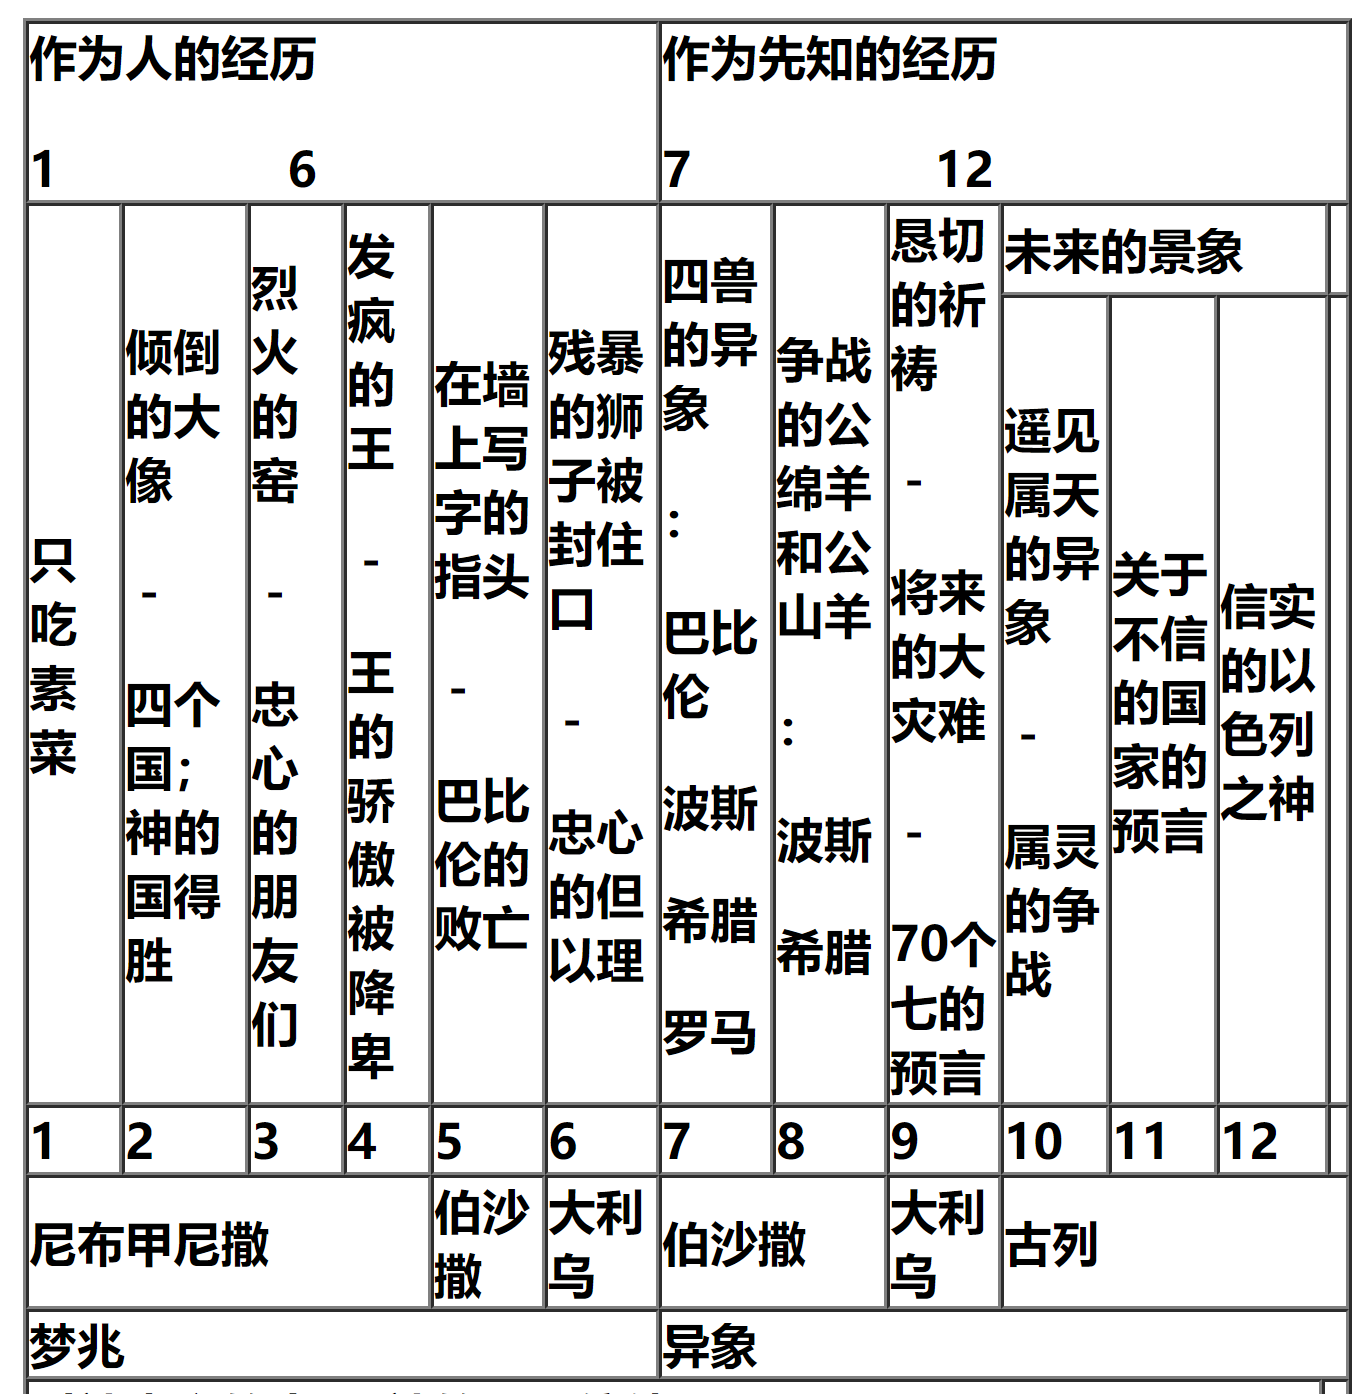
\includegraphics[width=6.in]{DXianZhiFigs/HeXiAFig/overall}
\caption{新城地界 1}
\label{fig:sub1}
\end{figure}

\begin{figure}%{.5\linewidth}
\centering
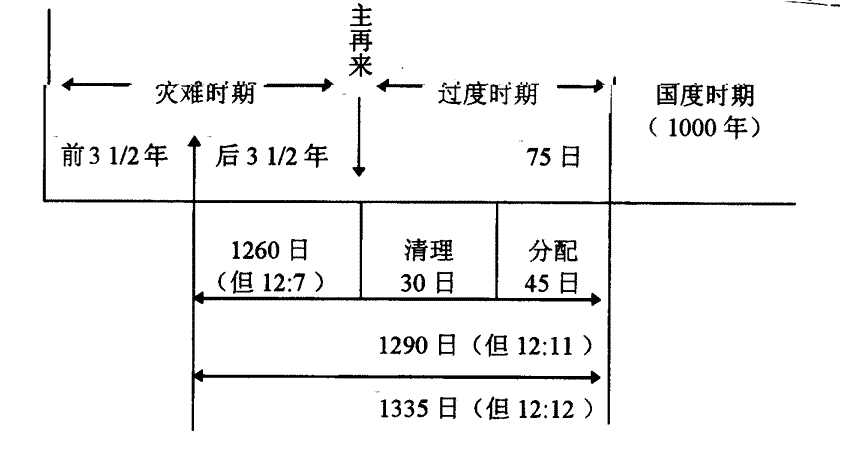
\includegraphics[width=6.in]{DXianZhiFigs/HeXiAFig/data}
\caption{新城地界 1}
\label{fig:sub1}
\end{figure}
\fi
%http://www.jonahome.net/files02/PI_Commentary-NTSurvey/gb/index.htm
%http://www.jonahome.net/files02/PI_Commentary-Dan/gb/11.htm
%http://www.jonahome.net/files02/PI_Commentary-Dan/gb/index.htm























